\renewcommand{\theequation}{\theenumi}
\begin{enumerate}[label=\arabic*.,ref=\thesubsection.\theenumi]
\numberwithin{equation}{enumi}
\item  given that $\to$
\begin{align}
Z &= 3x + 5y
\\
\text{subjected to}
\\
x + 3y &\geq 3
\\
x + y &\geq 2
\\
x  &\geq 0
\\
y &\geq 0
\end{align}
Comparing above equation to the gernelised form$\to$ 
\begin{align}
minZ &= c^t \vec{x}
\\
\text{subjected to}
\\
A\vec{x} &\preceq b
\\ 
\text{we can find $\to$ }
\\
c &= \myvec{3\\ 5}
\\
A &= \myvec{3 & 5 \\ 1 & 1}
\\
b &= \myvec{3\\2}
\end{align}\\
Solution for the above equations can be find from the python code of Lenear programing.\\
\begin{lstlisting}
./optimization/codes/lp6.eps
\end{lstlisting}
From the codes we get that the miniimum value of the equation will be 7 at the point $\myvec{1.5 & 0.5}$.

\begin{figure}[!ht]
	\centering
	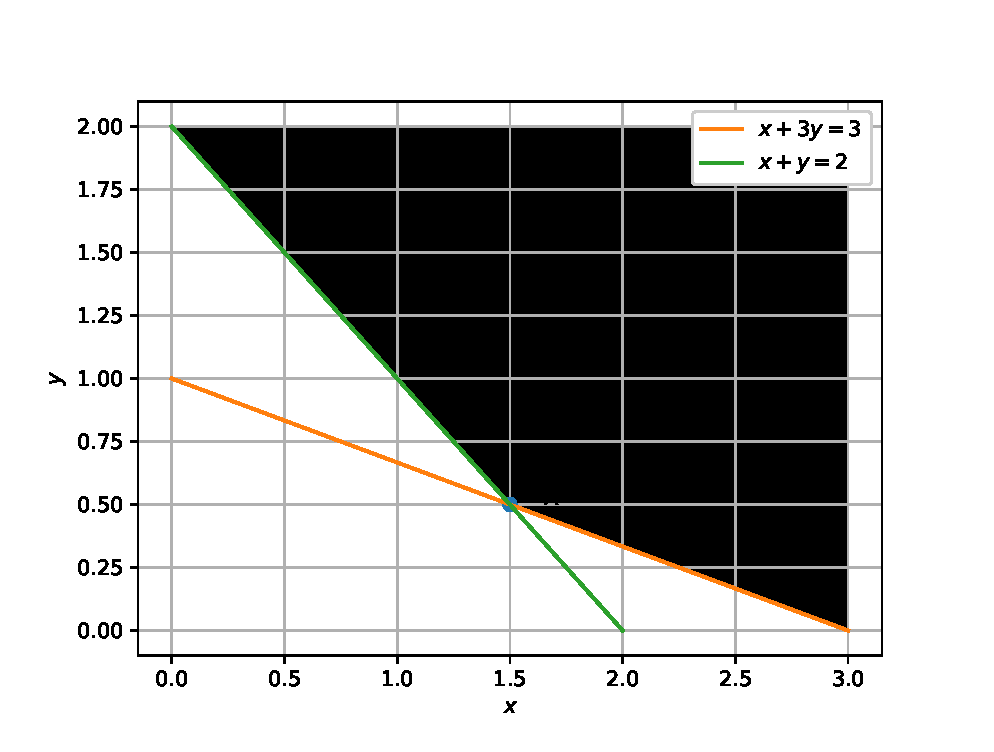
\includegraphics[width=\columnwidth]{./figures/lp6.eps}
	\caption{ lp6}
	\label{fig:lp6}
	pythone codes for the above figure can be get from
	\begin{lstlisting}
	./optimization/figures/lp6.eps
	\end{lstlisting}	
\end{figure}

\end{enumerate}